\section{Modell}
Als Modell wird ein Klassifizierer bezeichnet, das mit ML konstruiert wurde. In diesem Fall besteht der Klassifizierer aus Entscheidungsbäumen. Jede Konfiguration eines Modells besteht aus einer
Ensemble-Methode, einer Feature-Menge und Hyperparametern. Die Hyperparameter bestimmen die maximale Baumhöhe, die Waldgröße und die Blattgröße.
\newline
\newline
Jede Konfiguration wird mit dem in Abbildung \ref{fig:model_workflow} illustrierten Arbeitsablauf verarbeitet. Zunächst werden die Rohdaten verarbeitet, wobei eine beschriftete Trainingsmenge mit der definierten
Feature-Menge extrahiert wird. Dann wird das Modell trainiert und als C-Code exportiert. Der C-Code wird mit \textit{GCC} kompiliert, wodurch der C-Code zu einem ausführbaren Programm konvertiert wird. Das Programm
wird anschließend mit dem Werkzeug \texttt{Simulator} auf den definierten Trainingsmengen validiert.
\begin{figure}
    \centering
    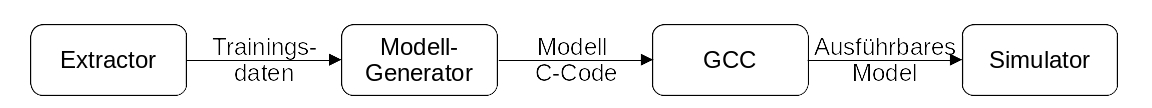
\includegraphics[width=\linewidth]{images/model_workflow.jpg}
    \caption{Arbeitsablauf, um ein Modell zu trainieren und zu validieren.}
    \label{fig:model_workflow}
\end{figure}

\subsection{Training}
\label{sec:Training}
Das Modell wird mit \textit{Scikit-Learn} trainiert. Die Konstruktion eines Entscheidungsbaumes ist aber nicht deterministisch, da es bei der Konstruktion mit CART Teilungen geben kann, die gleich gut sind
(Kapitel \ref{sec:construction}). In diesem Fall wählt Scikit-Learn zufällig eine Teilung aus. Dies beeinflusst die folgenden Teilungen und somit die Klassifizierungsgenauigkeit auf der
Trainings- und Testmenge. Der Zufall kann gesteuert werden, indem der Startwert des Zufallsgenerators auf einen vordefinierten Wert gesetzt wird. Mit einem konstanten Startwert ist Scikit-Learn deterministisch.
\newline
\newline
Daraus folgt, dass einige Startwerte bessere Modelle erzeugen als andere, obwohl die Konfiguration identisch ist. Folglich wurde festgestellt, dass die Konstruktion mit Scikit-Learn als Monte Carlo Methode verstanden
werden kann. Durch wiederholtes Trainieren mit unterschiedlichen Startwerten, erhöht sich die Wahrscheinlichkeit, dass das beste Modell gefunden wurde. Aus diesem Grund wird das
Modell mit 140 verschiedenen Startwerten für den Zufallsgenerator trainiert. Beim manuellen testen wurden im schlechtesten Fall nach 138 verschiedenen Startwerten keine Verbesserungen im Modell mehr festgestellt,
weswegen sich für etwas mehr, d. h. 140, entschieden wurde.
\newline
\newline
Um die 140 Modelle der gleichen Konfiguration miteinander zu vergleichen, wurde die Trainingsmenge zufällig in zwei Mengen unterteilt. Die eine Hälfte wurde zum Trainieren des Modells verwendet und die andere
Hälfte wurde zum Validieren des Modells verwendet. Aus den 140 trainierten Modellen wurde das Modell mit der höchsten Klassifizierungsgenauigkeit auf der Validationsmenge ausgewählt.
\newline
\newline
Es wurde jede Ensemble-Methode getestet, die in Kapitel \ref{sec:Ensemble} genannt wurde und mit dem Wahlklassifizier zusammengefasst. Die Waldgrößen sind zwischen 1 und 16, die maximalen Baumhöhen zwischen
1 und 22 und die Blattgrößen 1, 2, 4 oder 8.

\subsection{C-Code Generierung eines Entscheidungsbaumes}
\label{sec:cCodeTree}
Zur Ausführung eines Entscheidungsbaumes wird C-Code erzeugt. Dies ist erforderlich, weil der Entscheidungsbaum auf einem kleinen eingebetteten System ausgeführt werden soll. Die Toolchain, um die Firmware
dafür zu generieren, bedarf meistens, dass der Quellcode in der Programmiersprache \texttt{C} implementiert ist. Dies trifft auch auf das für dieses Projekt verwendete Arduino Board ATmega328P zu.
\newline
\newline
Für jeden Entscheidungsbaum wird eine Funktion generiert. Listing \ref{lst:sklearnCCodeTreeFunction} zeigt den Funktionskopf eines Entscheidungsbaumes. Als Eingabe wird ein Zeiger auf die Feature-Menge
\texttt{features} übergeben und ein Zeiger auf das Rückgabe-Array \texttt{result}, dass die Wahrscheinlichkeitsverteilung des Entscheidungsbaumes als Ergebnis speichert.
\begin{lstlisting}[label=lst:sklearnCCodeTreeFunction,caption={C-Code Funktionskopf eines Baumes $i$.}]
void tree_i(float* features, float* result);
\end{lstlisting}
Das Modell, dass von Scikit-Learn generiert wird, hat eine interne Datenstruktur, um den Entscheidungsbaum darzustellen. Aus dieser Datenstruktur wird der C-Code generiert. Listing
\ref{lst:sklearnTreeStructure} skizziert eine vereinfachte Darstellung dieser Datenstruktur, wobei \texttt{T} der Datentyp der Feature-Menge ist. Jeder Knoten ist entweder ein Blattknoten oder
ein innerer Knoten. Jeder Blattknoten beinhaltet die Wahrscheinlichkeitsverteilung, mit der jede Klasse in diesem Knoten anzutreffen ist. Jeder innere Knoten verfügt über einen Schwellenwert und
den Index zum Feature, dass er nutzt, um im Test den Schwellenwert mit dem Feature zu vergleichen. Außerdem enthält er seine Kindknoten. Scikit-Learn konstruiert binäre Entscheidungsbäume,
weswegen es genau zwei Kindknoten gibt.
\begin{lstlisting}[label=lst:sklearnTreeStructure,caption={Vereinfachte Datenstruktur von Scikit-Learn für Entscheidungsbäume.}]
enum Knoten<T> {
    Blattknoten {
        klassen_wahrscheinlichkeiten: Vec<f64>
    },
    InnererKnoten {
        feature_index: usize,
        schwellenwert: T,
        knoten_links: Knoten<T>,
        knoten_rechts: Knoten<T>
    }
}
\end{lstlisting}
Listing \ref{lst:sklearnCCodeParent} zeigt den C-Code, der für einen inneren Knoten generiert wird. Von der Wurzel aus, wird bis zu einem Blattknoten traversiert. Dabei wird rekursiv für jeden inneren
Knoten ein \texttt{if (Test) \{ \ldots\ \} else \{ \ldots\ \}} Ausdruck generiert. Der \textit{Test} ist ein Vergleich des ausgewählten Features und einem Schwellenwert. Aus der Feature-Menge \texttt{features}
wird das Feature an der Stelle \texttt{feature\_index} mit dem \texttt{schwellenwert} verglichen. Im Fall, indem der Ausdruck wahr ist wird der linke Kindknoten traversiert, ansonsten der rechte Kindknoten.
Die Ausdrücke \texttt{feature\_index} und \texttt{schwellenwert} werden im in Listing \ref{lst:sklearnCCodeParent} durch die in der Datenstruktur eines inneren Knotens vorzufindenden Konstanten ersetzt.
\begin{lstlisting}[label=lst:sklearnCCodeParent,caption={C-Code eines inneren Knotens.}]
if (features[feature_index] <= schwellenwert) {
    Traversiere Kindknoten links...
} else {
    Traversiere Kindknoten rechts...
}
\end{lstlisting}
Für einen Blattknoten muss der C-Code für die Rückgabe generiert werden. Listing \ref{lst:sklearnCCodeLeaf} zeigt, dass im Rückgabeparameter \texttt{result} für alle $M$~Klassen die Wahrscheinlichkeit
jeder Klasse gespeichert wird. Diese Rückgabe ist notwendig, da der Wahlklassifizierer, der diese Funktion ausführt, eine Wahrscheinlichkeitsverteilung erwartet.
Die Ausdrücke \texttt{klassen\_wahrscheinlichkeiten[i]} werden durch die Konstanten ersetzt, die in dieser Variable in der Datenstruktur eines Blattknotens gespeichert sind.
\begin{lstlisting}[label=lst:sklearnCCodeLeaf,caption={C-Code eines Blattknotens.}]
result[0] = klassen_wahrscheinlichkeiten[0];
...
result[M - 1] = klassen_wahrscheinlichkeiten[M-1];
return;
\end{lstlisting}

\subsection{C-Code Generierung eines Entscheidungswaldes}
Ein Entscheidungswald besteht aus einem Ensemble von Entscheidungsbäumen. Bei der Ausführung eines Entscheidungswaldes wird jeder enthaltende Entscheidungsbaum ausgeführt. Die Ergebnisse jedes
Entscheidungsbaumes werden mit dem Wahlklassifizierer (Kapitel \ref{sec:wahlklassifizierer}) zusammengefasst. Das heißt, die Wahrscheinlichkeiten jeder Klasse werden addiert und die Klasse mit
der größten Summe wird ausgewählt.
\newline
\newline
Listing \ref{lst:sklearnCCodeTreeVoting} zeigt den C-Code, der zum Zusammenfassen eines Entscheidungswaldes mit einem Wahlklassifizierer generiert wird. Zunächst wird ein
Array \texttt{total\_res} erstellt, dass die Summe der Ergebnisse der einzelnen Entscheidungsbäume speichert. Die Anzahl der Ergebnisse pro Entscheidungsbaum, d. h. die Anzahl an Rückgabeklassen, ist $M$.
Als Speicher für die Ergebnisse eines Entscheidungsbaumes wird \texttt{tree\_res} erstellt. In Zeile 6-9 wird ein Entscheidungsbaum $i$ ausgeführt und sein Rückgabe wert auf \texttt{total\_res} addiert.
Dieser Codeblock wird für alle $N$ Entscheidungsbäume wiederholt, die im Entscheidungswald enthalten sind. In Zeile 11-18 wird die Klasse ermittelt, die die höchste summierte Wahrscheinlichkeit hat.
In Zeile 19 wird die Klasse an die aufrufende Funktion zurückgegeben.
\begin{lstlisting}[label=lst:sklearnCCodeTreeVoting,caption={C-Code des Wahlklassifizierers mit $M$ Klassen und $N$ Bäumen.}]
01: unsigned char execute_decision_forest(float* features) {
02:     float total_res[M] = { 0.0, ..., 0.0 };
03:     float tree_res[M] = { 0.0, ..., 0.0 };
04:
05:     // Die folgenden 4 Zeilen werden für alle N Bäume wiederholt.
06:     tree_i(features, tree_res);
07:     total_res[0] += tree_res[0];
08:     ...
09:     total_res[M-1] += tree_res[M-1];
10:
11:     unsigned char max_index = 0;
12:     float max_value = 0;
13:     for (unsigned char i = 0; i < M; ++i) {
14:         if (max_value < total_res[i]) {
15:             max_value = total_res[i];
16:             max_index = i;
17:         }
18:     }
19:     return max_index;
20: }
\end{lstlisting}